% ---------------------------------------------------------------------------
\section{Deployment}
\label{sec:deployment}
% ---------------------------------------------------------------------------

\subsection{Architecture and API contract}

The system has three runtime components (Table~\ref{tab:components}). The inference
service is a FastAPI application that loads the serialised pipeline at start-up and
exposes point estimates, intervals, batch scoring, local explanations and the latest
monitoring summary. The valuation console is a Streamlit application \citep{streamlit2026} that renders
a listing form for agents and a read-only monitoring view. Monitoring artefacts are
generated offline by a scheduled script and served both as a static HTML dashboard
and through the API, so the console never computes statistics itself.

\begin{table}[htbp]
\centering
\caption{Runtime components of the deployed valuation product. Paths are relative to
the repository root.}
\label{tab:components}
\small
\begin{tabularx}{\linewidth}{@{}L{0.16\linewidth}L{0.32\linewidth}L{0.07\linewidth}X@{}}
\toprule
\textbf{Component} & \textbf{Entry point} & \textbf{Port} & \textbf{Purpose} \\
\midrule
Valuation API & \path{src/revaluation/api/main.py} & 8000 & Estimates, intervals, batch scoring, explanations, monitoring summary \\
Valuation console & \path{app/streamlit_app.py} & 8501 & Agent-facing form, performance and monitoring views \\
Monitoring artefacts & \path{scripts/06_run_monitoring.py} & --- & Drift report, alerts, static HTML dashboard \\
\bottomrule
\end{tabularx}
\end{table}

Two design decisions matter. The API is stateless apart from the model artefact, so
it scales horizontally without session affinity. The console calls the API through
the \texttt{VALUATION\_API\_URL} variable but falls back to an in-process copy of the
same pipeline when the API is unreachable, which keeps a single-service deployment
demonstrable on free tiers where a sleeping API would make the console appear broken;
both paths use the identical pipeline object, so the fallback cannot diverge in
preprocessing.

Table~\ref{tab:endpoints} lists the interface. Validation is declarative through
Pydantic models, and only four fields are required: neighbourhood, overall quality,
above-grade living area and year built. Every other field has a documented default,
so an agent can obtain an estimate from an incomplete listing rather than being
blocked by a long form, and the response records which assumptions were applied.

\begin{table}[htbp]
\centering
\caption{HTTP interface of the valuation API. Interactive OpenAPI documentation is
served at \texttt{/docs} by the framework \citep{fastapi2026}.}
\label{tab:endpoints}
\small
\begin{tabularx}{\linewidth}{@{}L{0.09\linewidth}L{0.25\linewidth}X@{}}
\toprule
\textbf{Method} & \textbf{Path} & \textbf{Purpose} \\
\midrule
GET & \texttt{/health} & Liveness plus model-loaded flag \\
GET & \texttt{/model/info} & Model card, version and validation metrics \\
POST & \texttt{/predict} & Point estimate, 80 and 90 per cent intervals, confidence class \\
POST & \texttt{/predict/batch} & Up to 200 listing profiles per request \\
POST & \texttt{/explain} & Local SHAP contributions for one profile \\
GET & \texttt{/monitoring/summary} & Latest drift, performance and alert summary \\
\bottomrule
\end{tabularx}
\end{table}

The prediction response contains the estimate, both intervals, a confidence class, a
confidence score, the relative 90 per cent interval width, the model name and version,
the assumptions applied and a timestamp. The class is derived from the relative
half-width of the 90 per cent interval: at most 0.18 is high confidence, at most 0.30
is moderate, and anything wider is low and routed to a valuer, which implements the
escalation policy of Section~\ref{sec:business}. An exact request and response are
reproduced in Appendix~\ref{app:api}.

\subsection{The valuation console and packaging}

Figure~\ref{fig:console} shows the console after a request. Inputs are grouped into
location and transaction date, structure and condition, and an optional
neighbourhood-amenity section, so an agent who knows only the basics can still obtain
a valuation. The result panel reports the point estimate, both intervals and the
confidence assessment, and the lower panel lists the local contributions that moved
this particular estimate. For the illustrated profile, a 1975 house in CollgCr with
quality 6, condition 5, 1,500 square feet of living area and a 2005 remodelling, the
response is 146,412 \USD{} with an 80 per cent interval of 130,213--164,626 \USD, a
90 per cent interval of 124,164--172,646 \USD{} and a high confidence classification
with a score of 0.67.

\begin{figure}[htbp]
\centering
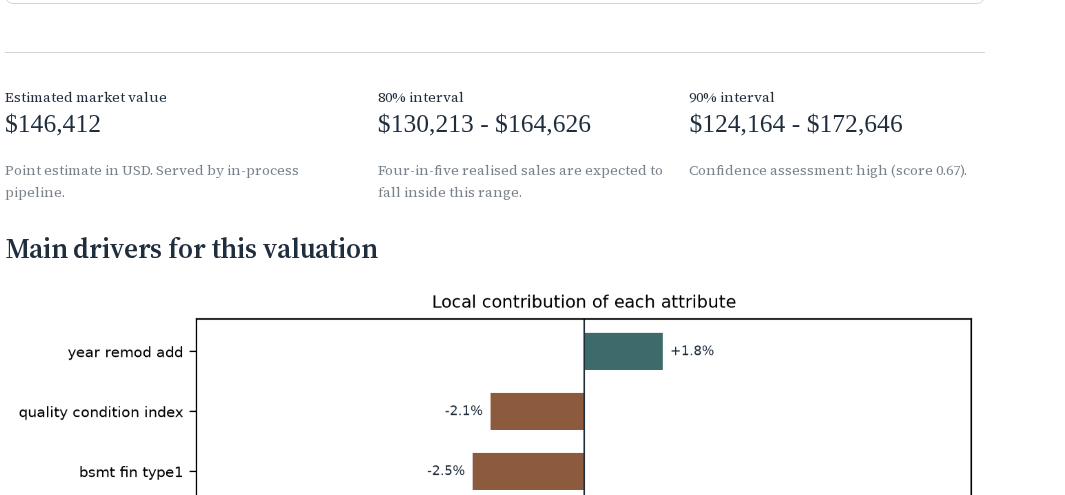
\includegraphics[width=0.95\linewidth]{ui_result_panel.png}
\caption{Result panel of the Streamlit valuation console after a request, cropped
from the full-window capture to keep the output legible. The panel reports the point
estimate with both conformal intervals, the confidence assessment and the local
attribution of the leading drivers.}
\label{fig:console}
\end{figure}

The console also provides a model-performance page and a monitoring page that read
the archived metrics and alerts, so a non-technical stakeholder can inspect the
evidence behind the numbers without opening a notebook. This matters for adoption:
the valuation is useful only if an agent can see how often it has been right.

Two container images are provided: the API image serves the application on the port
given by \texttt{PORT} (default 8000), and the console image does the same for
Streamlit on 8501. Neither trains a model at start-up, so cold starts are dominated
by process startup. A Compose file starts both services, a Render blueprint declares
the two web services with build commands and health checks, and a Hugging Face
Spaces variant uses the Docker SDK on port 7860. Both free tiers impose
sleep-on-inactivity behaviour and a 512 MB ceiling, which the system fits.

\subsection{Verification status and the public-URL question}

The complete system has been verified locally. The health endpoint returns a healthy
status with the model loaded, the information endpoint returns the model card, the
prediction endpoint returns the response in Appendix~\ref{app:api}, the batch and
explanation endpoints return well-formed payloads, and the monitoring endpoint
returns the latest summary once the monitoring script has run. The console renders
the form, calls the service, displays the intervals and the local attribution, and
the static monitoring dashboard is generated without error.

No public URL is claimed. The Render blueprint and the Hugging Face configuration are
complete and the procedure is documented, but provisioning either service requires
the account credentials of the repository owner, which were not available in the
development environment. The team chose not to publish a link that could not be kept
alive, and this report does not present a local address as if it were public. The
remaining work is administrative: authenticate to the hosting account, connect the
repository, set \texttt{VALUATION\_API\_URL} on the console service and confirm the
health check. Until that is done, the deployment criterion of the brief is satisfied
in substance but not in form, and the report states this plainly rather than implying
otherwise.
